\chapter{EvoOracle: LLMs for Oracles}
\label{cha:evoOracles}
\vspace{0.4 cm}

In this chapter, we introduce EvoOracle, our proposed approach designed for potential oracle generation using Large Language Models and describe how the components of the approach have been implemented. 

\section{Proposed Approach}
\label{sec:approach}
\vspace{0.2 cm}

To commence the procedure, EvoOracle necessitates an initial preprocessing phase, which encompasses project analysis, source code parsing, and extraction of essential information essential for the subsequent generation process. The classes and tests undergo a systematic traversal across the tool's integrated components to yield an accurate Oracle. EvoOracle's architecture incorporates several interworking components that collaboratively generate test cases and oracles for designated projects. The illustration in Figure ~\ref{fig:component_diagram} furnishes a comprehensive overview of the key components within EvoOracle. Each of the components are explained in details below:

\begin{figure}[H]
\centering
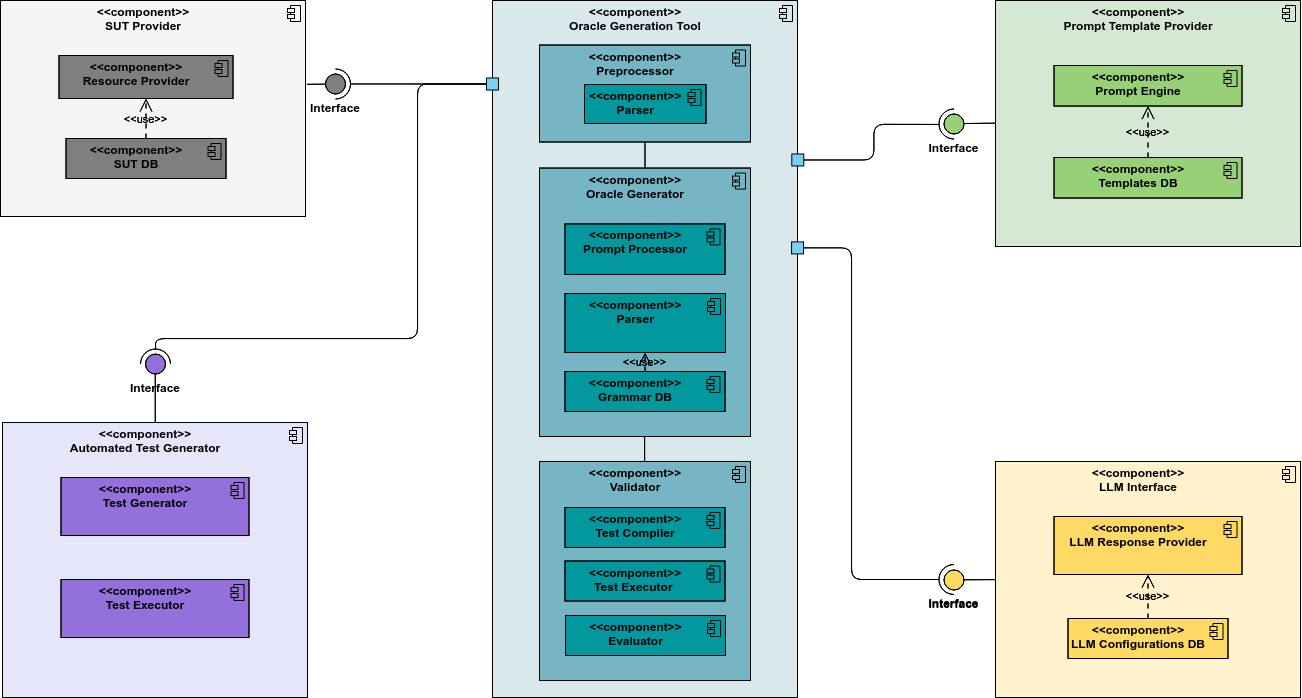
\includegraphics[width=1\textwidth]{images/EvoOracle_ components.png}
\caption{Components of our proposed approach: EvoOracle}
\label{fig:component_diagram}
\end{figure}

\begin{enumerate}
    \item \textbf{Preprocessor:} The Preprocessor is a fundamental component that analyzes the System Under Test (SUT) by parsing its code. It systematically examines each project, extracting vital details about classes and methods, along with their associated metadata. Additionally, the component identifies and establishes connections with test classes generated by the automated test generation component. It facilitates mapping each test case within a test class to the corresponding focal method. The preprocessor incorporates a parser component, which plays a pivotal role in extracting metadata linked to identified classes and methods. By traversing the project folder and locating source files, the parser parses each class file into an Abstract Syntax Tree (AST). This process collects essential information such as class names, signatures, superclasses, bodies, annotations, interfaces, package details, imports, fields, arguments list, constructors, dependencies and variables, method names, return types, and any developer-written comments. While navigating the AST, EvoOracle gathers information at both class and method levels. This parsed code serves a dual purpose: pinpointing test cases and their corresponding focal methods, and enhancing focal methods by incorporating contextual information.
    
    \item \textbf{Oracle Generator:} The Oracle Generator is a critical component responsible for processing test cases generated by the Automated Test Generator. This generator produces a test suite for each target class, considering criteria like line coverage, branch coverage, configuration, and budget. With the inclusion of placeholders and focal methods, it prepares the context for LLM prompting. The Oracle Generator adopts a two-step approach, employing specific heuristics to preprocess test cases. This ensures that the test cases are adequately prepared for assertion generation, following these steps:

    \begin{enumerate}
        \item \textbf{Removal of Assertions:} All selected test cases undergo the removal of assertions, retaining only the last assertion in case there are multiple assertions using Algorithm~\ref{algorithm_remove_assertion}. This decision is based on the likelihood that reaching the last assertion implies satisfaction of all preceding assertions. This is a reasonable choice which is also seen in the work of Tufano et al. \cite{tufano_generating_2022}. The purpose is to streamline the test cases for further processing.

        \item \textbf{Placeholder Insertion:} Following the removal of additional assertions, the test cases are left with a single assertion. We replace this single assertion with a placeholder using Algorithm~\ref{algorithm_placeholder_insertion}. This placeholder serves as a temporary marker and will be subsequently replaced with assertions generated by the Large Language Models.

        \item \textbf{Prompt Templates:} This component utilizes prompt templates in creating a focal context tailored for each Class Under Test (CUT) and its corresponding Method Under Test (MUT). These templates serve as the foundation for replacing the contextual placeholders with the specific contexts of interest. This dynamic approach ensures that the LLMs receive targeted and meaningful prompts, enhancing their understanding of the given code context and enabling them to generate assertions with precision.

        \item \textbf{Prompt Generation Algorithm:} To create effective prompts for the Large Language Models, this component gathers information to build the context for a test case that was prepared in the preprocessing phase. This information includes key details about the class under test, methods under test, and various method attributes such as Constructor signature, Class Signature, parameters, Invoked Method Signature, dependencies, return type, developer comments, source code for the test case, package, imports, Fields, and getter/setter signature. We carefully consider all invoked methods and dependencies encapsulated within the test case. To improve the Oracles generated by the automated test generation tools, we propose the inclusion of LLMs into the test generation process. LLM Interface component provides empowers developers to tailor their LLM choices, ensuring compatibility and aligning with their project requirements and provides response. In instances where the LLM response faces challenges such as token limit exceeds, we dynamically adjust the context size. An iterative process is followed as shown in Algorithm~\ref{algorithm_prompt_generation} of generating prompts for the LLM, involving multiple rounds. Each round refines the prompt based on the LLM's response and aims to address potential challenges like token limit exceedance. The trimming process, controlled by conditional statements, adjusts the size of critical elements such as method details and test method code. This adaptive approach ensures that the prompt remains concise while retaining essential contextual information. The code systematically handles different trimming scenarios in each round, progressively refining the prompt to strike a balance between informativeness and LLM response feasibility. The overall mechanism involves generating messages from prompt templates, seeking LLM responses, and dynamically adjusting the prompt for subsequent iterations, all of which contribute to an effective and tailored interaction with the LLM.

        \begin{algorithm}
        \caption{Algorithm for \texttt{Removing all assertions but last}}
        \label{algorithm_remove_assertion}
        \begin{algorithmic}[1]
        \Function{remove\_all\_assertions\_but\_last}{$\text{source\_code}$}
            \State $\text{assertion\_patterns} \gets$ [\texttt{...}] \Comment{List of assertion patterns}
            \State $\text{assertions} \gets \text{FIND ALL(assertion\_pattern, source\_code)}$
        
            \If{\text{NO assertions}}
                \State \textbf{return} $\text{source\_code}$
            \EndIf
        
            \State $\text{replaced\_assertions} \gets []$
        
            \For{$i$ \textbf{in} \text{range}(\text{len(assertions) - 1})}
                \State $\text{source\_code} \gets \text{SUBSTITUTE (assertion\_pattern, "", source\_code, count=1)}$
                % \State $\text{replaced\_assertions.append(assertions[i][0] + assertions[i][1] + "();")}$  % Uncomment this line if you want to keep track of removed assertions
            \EndFor
        
            \State \textbf{return} $\text{source\_code}$
        \EndFunction
        \end{algorithmic}
        \end{algorithm}
        
        \begin{algorithm}
        \caption{Algorithm for \texttt{Placeholder insertion}}
        \label{algorithm_placeholder_insertion}
        \begin{algorithmic}[1]
        \Function{replace\_assertions}{$\text{source\_code}$}
            \State $\text{assertion\_patterns} \gets$ [\texttt{...}] \Comment{List of assertion patterns}
            \State $\text{replaced\_assertions} \gets$ [] \Comment{List to store replaced assertions}
        
            \For{$\text{pattern}$ \textbf{in} $\text{assertion\_patterns}$}
                \Function{replacement}{$\text{match}$}
                    \State $\text{matched\_text} \gets \text{TRY MATCH}$
                    \State $\text{replaced\_assertions.append(matched\_text)}$
                    \State \textbf{return} \texttt{(ASSERTION\_PLACEHOLDER)}
                \EndFunction
        
                \State $\text{source\_code} \gets \text{SUBSTITUTE (pattern, replacement, source\_code)}$
            \EndFor
        
            \State \textbf{return} $\text{source\_code, replaced\_assertions}$
        \EndFunction
        \end{algorithmic}
        \end{algorithm}
        
        \begin{algorithm}
            \caption{Prompt Generation Algorithm}
            \label{algorithm_prompt_generation}
            \begin{algorithmic}[1]
                \Function{generate\_prompt}{$\text{context}$}
                    \State $\text{rounds}, \text{max\_attempts}, \text{prompt\_template} \gets []$ \Comment{No. of Iterations, attempts, prompt template}
                    \State $\text{prompts\_and\_responses} \gets []$
                    
                    \While{$\text{rounds} < \text{max\_attempts}$}
                        \State $\text{steps}, \text{rounds} \gets 0, \text{rounds} + 1$
                        \If{$\text{rounds} > 2$}
                            \State $\text{trimmed\_context} \gets \text{trim\_context(context, 3)}$ \Comment{Trim context by reducing Method depth}
                        \EndIf
                        
                        \If{$\text{rounds} > 1$}
                            \State $\text{trimmed\_context} \gets \text{trim\_context(context, 5)}$ \Comment{Trim context by reducing Method depth}
                        \EndIf
                        
                        \State $\text{messages} \gets \text{generate\_messages(prompt\_template, trimmed\_context)}$
                        
                        \State $\text{llm\_result} \gets \text{ask\_openLLM(messages)}$
                        \State $\text{prompts\_and\_responses.append(\{"prompt": messages, "response": llm\_result\})}$
                        
                        \State $\text{source\_code, replaced\_assertions} \gets \text{replace\_assertions(source\_code)}$
                        
                        \If{$\text{assertions}$ NOT GENERATED}
                            \State $\text{context} \gets \text{update\_prompt\_and\_ask\_again(context)}$
                        \EndIf
                    \EndWhile
                    
                    \State $\text{print\_and\_save\_results(prompts\_and\_responses)}$
                \EndFunction
            \end{algorithmic}
        \end{algorithm}
        
        Throughout each iteration, we analyze LLM responses to capture assertions using the specified Assertion regex. When the parsing operation successfully identifies an assertion, we advance to the subsequent phase of crafting the test case with EvoOracle assertion. In cases where the assertion parsing is unsuccessful, we continue the iteration process until we reach the budget limit specified in the configuration. 
    \end{enumerate}

    \begin{figure}[H]
    \centering
    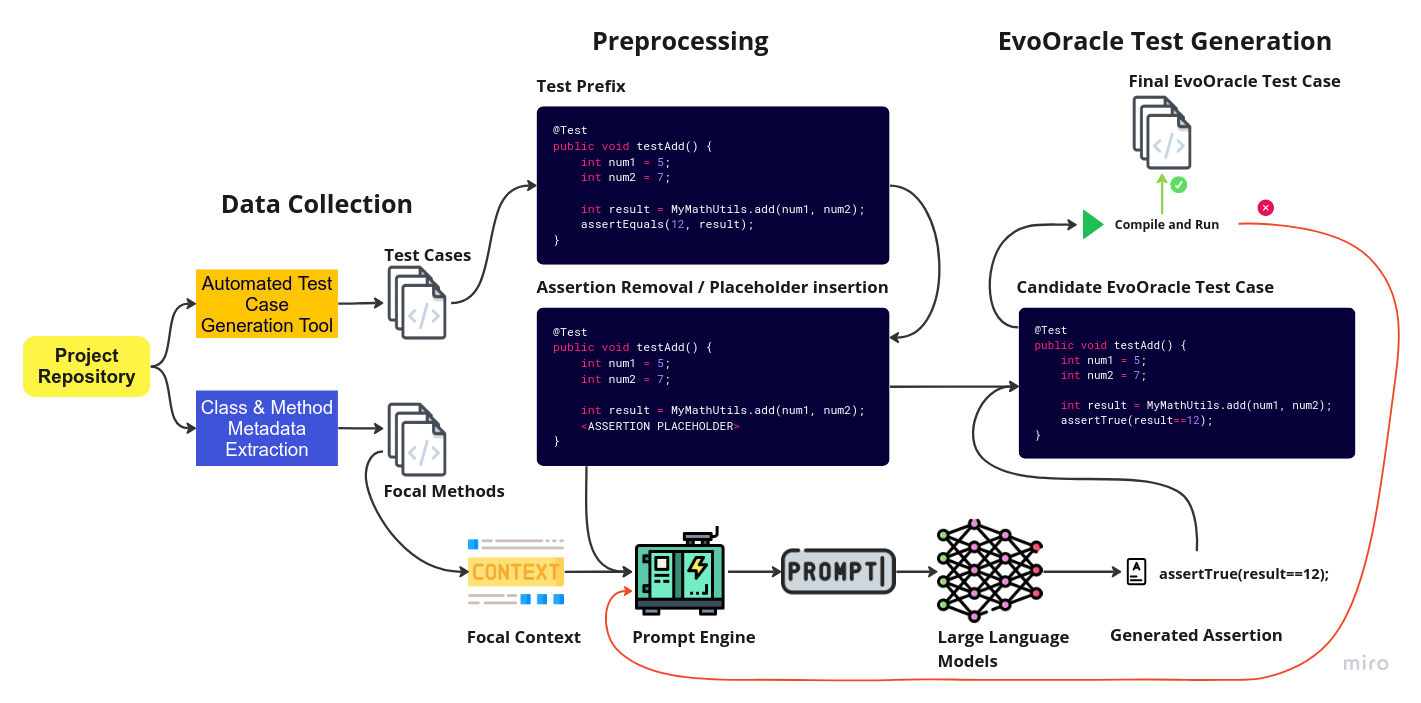
\includegraphics[width=1\linewidth]{images/evooracle_overview.png}
    \caption{Overview of EvoOracle}
    \label{fig:evooracle_overview}
    \end{figure}

    \item \textbf{Validator:} This component follows heuristics to evaluate the quality of the generated tests. After receiving a response from LLM interface, EvoOracle extracts and validates the assertions while selecting a different prompt modifications if any errors are detected during the validation process. 
    \\
    \textbf{Extract:} We follow a generalized approach for extracting tests from responses. EvoOracle employs regular expressions to identify strings that matches with a set of predefined assertion formats. If EvoOracle fails to extract any assertions from LLM’s response, the whole process starts again for the next attempt with a modified prompt. Otherwise, it is considered that there is no syntactic error and the assertion is replaced back from the test case we prepared earlier.
    \\
    \textbf{Compile and run:} In this step, EvoOracle compiles and executes the test. If the test fails to compile or encounters errors during execution, it proceeds to the next attempt. A test is considered passed only if it is free from syntax errors, compiles successfully, runs without errors.
    \\
    \textbf{Mutation testing:} If a test compiles and runs without any errors, it is already an indication that the candidate tests are good enough. Another criteria is to run mutation testing on the generated tests and select only those tests which has higher mutation score.
\end{enumerate}

Figure~\ref{fig:evooracle_overview} shows the overview of EvoOracle's components in action.

\section{Implementation}
\label{sec:implementation}
\vspace{0.2 cm}

The source code for our implementation of the tool can be found in the added references~\cite{evooracle_github}.
